%!TEX root = ../thesis.tex
\chapter{Conditionals}
\label{ch:Conditionals}


As of late a fair amount of work has gone into understanding exactly how the different frameworks handle conditionals.
This is of particular interest because the code generator generates conditionals in a certain form and we would like to understand how that is translated in each framework.

\section{Semantics of generated code}

Currently the code generator produces conditional code as seen in Figure~\ref{fig:generated-conditional-yauhau} for Yauhau and Figure~\ref{fig:generated-conditional-haxl} for Haxl.
From the Haxl example it is particularly obvious that values on both branches of the conditional are precomputed, that is the (monadic) operations necessary to compute both values are performed before the condition is being evaluated.
This has the consequence that any IO operation which is necessary to produce this value is performed before the condition for the \texttt{if} is evaluated and therefore might render the IO actions redundant if the value is not selected.
Of course the value might also be used in other, subsequent calculations, in which case precomputing is sensible.
In fact that is the reason why the graph serialisation in the code generator uses this particular style of code.
It does not inquire how many other nodes depend on the result of this calculation and hence obtains no evidence of whether it is safe move the computation onto the if branch itself.
As a recapture, we know now that the code generator produces conditional code for Haxl, were all branches are precomputed.
Following from the semantics of the Haxl framework all IO actions have already been performed on both values when the condition is evaluated and a branch is selected.

\begin{figure}
\begin{minted}{Clojure}
(let [val1 (computation ...)
      val2 (computation ...)]
  (if condition val1 val2))
\end{minted}
\caption{Generated conditional code for Yauhau}
\label{fig:generated-conditional-yauhau}
\begin{minted}{Haskell}
do
  (val1, val2) <- (,) <$> computation ... <*> computation ...
  return $ if condition then val1 else val2
\end{minted}
\caption{Generated conditional code for Haxl}
\label{fig:generated-conditional-haxl}
\end{figure}

\begin{figure}
  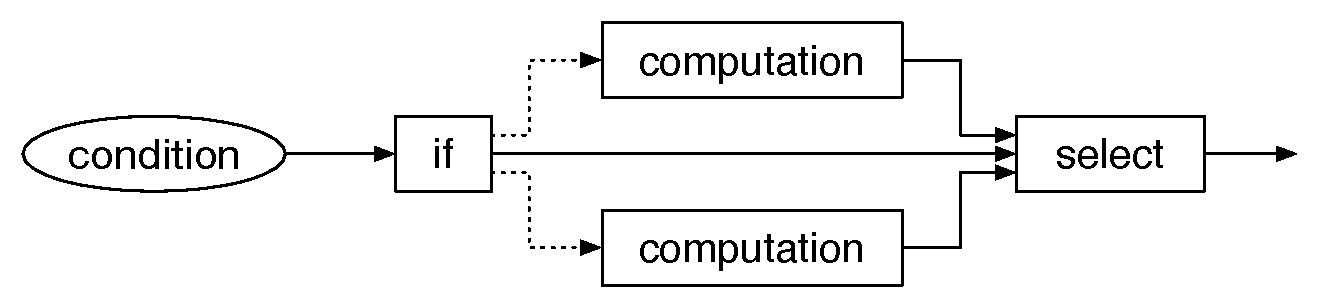
\includegraphics[width=\textwidth]{../Figures/if-hypothesised}
  \caption{Conditionals as hypothesised}
  \label{fig:if-graph-hypothesised}
  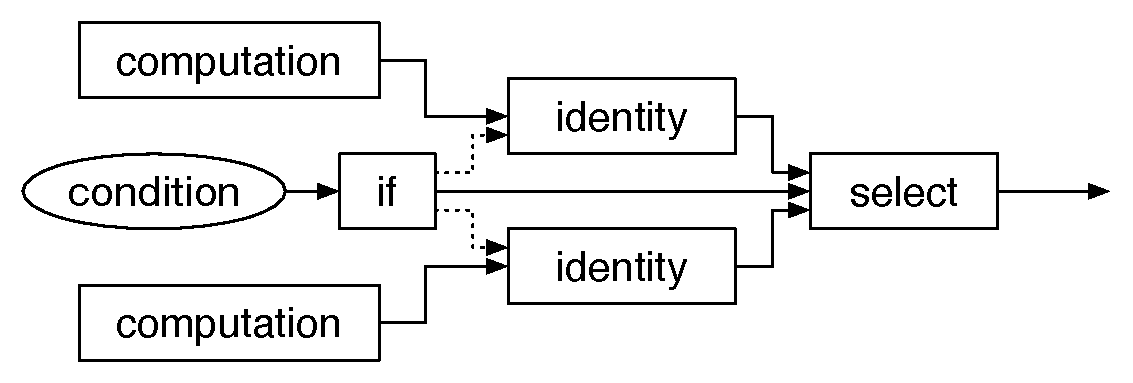
\includegraphics[width=\textwidth]{../Figures/if-in-reality}
  \caption{Conditionals actual}
  \label{fig:if-graph-actual}
\end{figure}

For a long time we suspected \yauhau{} and Ohua would handle this situation differently and \textbf{not} precompute the values, delay IO actions and only perform necessary calculations after evaluating the condition.
The reason we would come to this Hypothesis is because we thought operating on a dataflow graph would provide us with the necessary information and semantics by default.
However recently I discovered that, due to the way that Ohua translates code into graph, we do not in fact differ from Haxl in semantics.
As an example we will take the program from Figure~\ref{fig:generated-conditional-yauhau}.
We previously expected it to translate the program into a graph like the one in Figure~\ref{fig:if-graph-hypothesised}.
Here both computations are dependent on the \texttt{if} via a \textit{context arc} (dotted arrow) and therefore would be computed \textit{after} the condition had been evaluated.
The way in which Ohua would actually translate the program however would be to insert an operator called \texttt{value} on each of the if branches, which essentially wraps the bindings \texttt{val1} and \texttt{val2} respectively.
Additionally two \textit{context arcs} would be connected from the \texttt{if} to those \texttt{value} operators.
A visual representation of this can be seen in Figure~\ref{fig:if-graph-actual}.
At runtime, depending of the value of the condition, one of those \textit{context arcs} would be activated selecting the branch it is connected to, in this case the respective \texttt{value} operator.
In layman's terms the \texttt{if} selects one binding out of two at runtime, not one computation, as previously hypothesised.

We had also planned to show experiments later comparing the different semantics of \yauhau{} and Haxl when it comes to conditionals and discuss advantages and disadvantages of both.
Resulting from the recent unveilings however this has become redundant.
As much of a failure this may seem there is valuable information to be found in this.
Since we hypothesised these two different semantics we put additional thought into advantages and disadvantages of precomputing possibly unused values.


\section{Evaluation of precomputed conditional branches}

Let us assume that, in the system using Haxl or \yauhau{} computations are pure and the only stateful actions are the IO actions performed using the framework.
This view is of course not entirely consistent with reality, since nothing prevents you from doing effectful things in \yauhau{}, however in the domain where this system may be used it is a reasonable assumption to make for the purposes of the following deliberations.
Furthermore we may assume our fetches/reads to be \textit{pure} in so far as that they do not mutate the resource they request data from and serving a cached copy of a request is equivalent to actually performing the request.
How \yauhau{} deals with cases in which these assumptions do not hold is explained in detail in other chapters.

If we assume the mentioned, lets call it \textit{near purity}, we can start to consider code reordering as an optimisation.
In particular reordering code around conditional statements is a possible code optimisation.
It turns out that, when performing batching transformations, like we do, moving requests out of, or into conditional branches has more intricate and interesting effects than it would in a regular program.

Consider a simple example (Figure~\ref{fig:requests-on-branches}) where we have a regular conditional statement and depending on the result of the computation one request.
Consider how this program would be batched.
The requests on the branches depend on the the evaluation of the condition and the condition depends on the data from \texttt{request0}, see also Figure~\ref{fig:requests-on-branches-graph}.
Fetch rounds are indicated by the blue, dashed rectangle.
As a result we would end up with two fetch rounds.
One for the request before the conditional and one for either the request from the true branch or the false branch.

\begin{figure}
\begin{minted}{Clojure}
(let [data1 (get-data request0 source1)]
  (if (computation data1)
    (get-data request1 source1)
    (get-data request2 source2)))
\end{minted}
\caption{Requests on branches}
\label{fig:requests-on-branches}
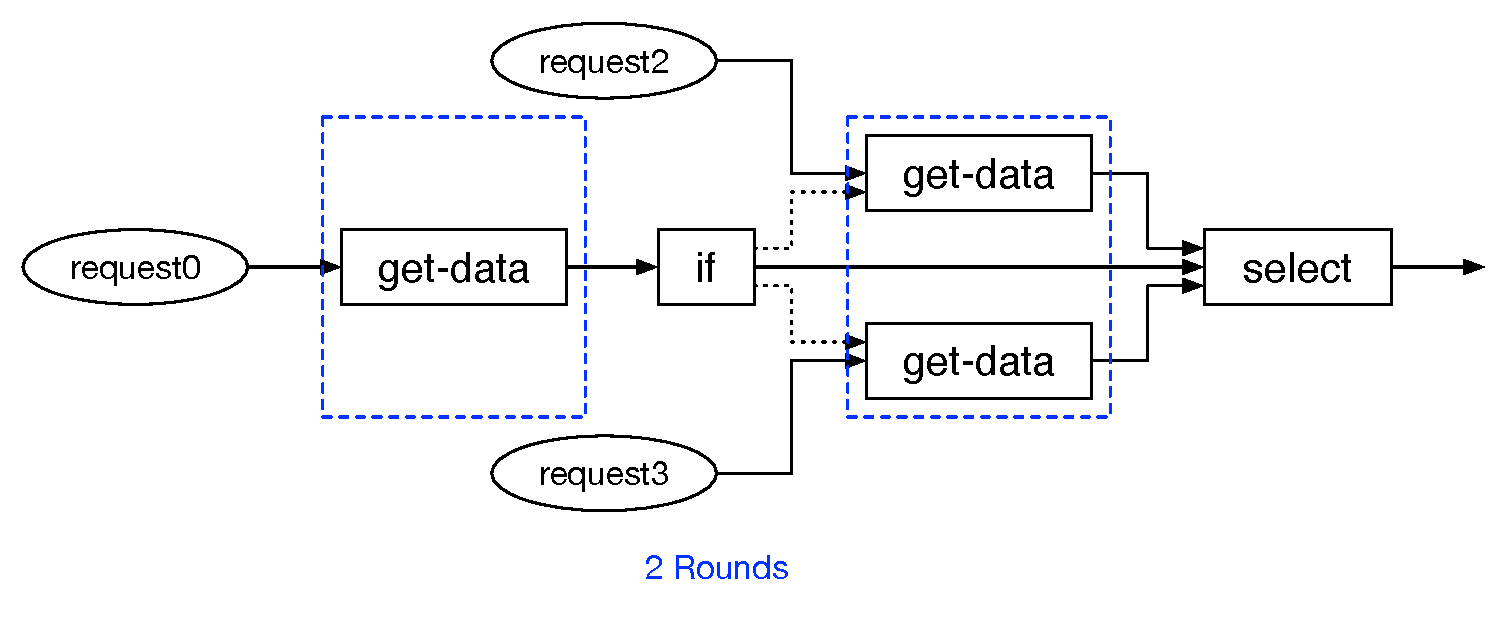
\includegraphics[width=\textwidth]{../Figures/requests-on-branches-graph}
\caption{Request on branches as graph}
\label{fig:requests-on-branches-graph}
\end{figure}

In \yauhau{} we generally operate under the assumption that IO actions are expensive.
The goal of our system is to do as few actual IO actions as possible.
In this case we see that we are performing two actions where we might only have to perform one action.
If we can, as previously mentioned, consider the fetches and computations as pure, we can rewrite the program to perform the conditional fetches \textbf{before} evaluating the condition (See Figure~\ref{fig:requests-precomputed}), which allows it to be batched with the first request, since the two fetches now do not depend on the condition anymore, See Figure~\ref{fig:requests-precomputed-graph}.
The round again indicated by the blue, dashed rectangle.
For pure computations this will be semantically identical even though it performs redundant computation.

\begin{figure}
\begin{minted}{Clojure}
(let [data1 (get-data request0 source1)
      data2 (get-data request1 source1)
      data3 (get-data request2 source2)]
  (if (computation data1)
    data2
    data3))
\end{minted}
\caption{Requests precomputed}
\label{fig:requests-precomputed}
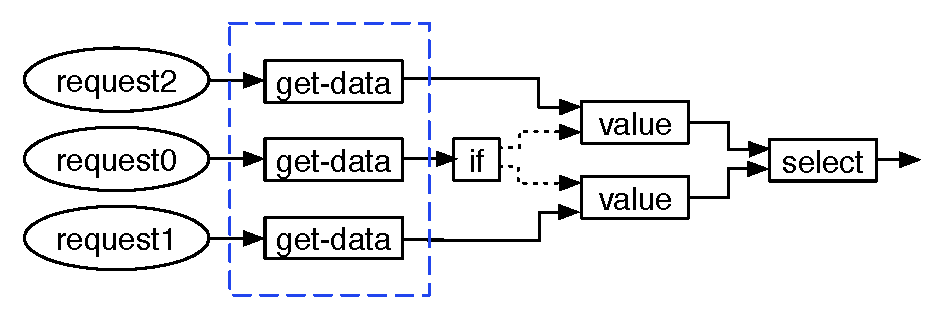
\includegraphics[width=\textwidth]{../Figures/requests-precomputed-graph}
\caption{Precomputed requests as graph}
\label{fig:requests-precomputed-graph}
\end{figure}

For many programs in our domain the latter version will be more efficient.
In particular if the fetch round before already includes a request to \texttt{source2} as well, then after our rewrite we get all the data from the entire second round for free.

However this is not always the case.
If the earlier round does not contain a request to \texttt{source2} already we would be performing an additional IO action.
It will run in parallel to the request to \texttt{source1} and thus seldom create additional latency, however if \texttt{source2} is significantly slower than \texttt{source1} our change could introduce a lot of additional latency into the program.

\begin{itemize}
  \item Rewrite from before branch to branch
  \item or rewrite from branch to precompute
  \item both require functions to be pure
  \item \texttt{@Pure} annotation?
\end{itemize}
